% Please make sure you insert your
% data according to the instructions in PoSauthmanual.pdf

\documentclass[a4paper]{PoS}
\usepackage{color}
\usepackage{graphicx}
\usepackage{apacite}
\usepackage{lineno}
\linenumbers

\title{Development and testing of a Trigger Processor Card based on a Kintex Ultrascale FPGA.}

\ShortTitle{Short Title for header}

%\author{\speaker{S. Mallios}, K. Adamidis, G. Bestintzanos\thanks{Univercity of Ioannina} \\
%        University of Ioannina\\
%        E-mail: \email{stavros.mallios@cern.ch}}
%
%\author{K. Adamidis, G. Bestintzanos, C. Fountas, G. Karathanasis, P. Katsoulis, N. Manthos, I. Papadopoulos, S. Sotiropoulos, P. Sphicas, C. Vellidis\\
%        Affiliation\\
%        E-mail: \email{...}}


\author{\speaker{S. Mallios}$ˆa$, S. Sotiropoulos$ˆ{b}$, K. Adamidis$ˆa$, G. Bestintzanos$ˆa$, C. Fountas$ˆa$, G. Karathanasis$ˆc$, P. Katsoulis$ˆa$, N. Manthos$ˆa$, I. Papadopoulos$ˆa$, S. Sotiropoulos$ˆb$, P. Sphicas$ˆc$, C. Vellidis$ˆc$\\
\llap{$ˆa$} University of Ioannina, Ioannina, Greece\\
\llap{$ˆb$} Institute of Accelerating Systems and Applications (IASA), Greece\\
\llap{$ˆc$} University of Athens, Athens, Greece\\
E-mail: \email{stavros.mallios@cern.ch@mail.org}}



%University of Ioannina1, University of Athens2 and Institute of Accelerating Systems and Applications (IASA), Athens3


\abstract{During the HL-LHC era , the upgraded detector will be read -out at an unprecedented data rate of up to 50Tb/s and an event rate of 750kHz. Within the scope of Phase-2 RD, a Level-1 Trigger processor card was designed, by the Greek CMS Trigger team, to provide a hardware environment for developing and evaluating new Level-1 trigger muon designs and technologies. The board is powered by a Kintex UltraScale FPGA . A new firmware was developed implementing 16Gbps links with IPbus support, to accommodate the testing of new algorithms. The hardware and firmware design of the board is presented here.}


\FullConference{Topical Workshop on Electronics for Particle Physics (TWEPP2018)\\
		17-21 September 2018\\
		Antwerp, Belgium}


\begin{document}

\pagenumbering{arabic}

\section{Introduction}
The upgraded High Luminosity LHC, after the third Long Shutdown (LS3), will provide an instantaneous luminosity of 7.5 10\^{}\{34\} cm\^{}\{-2\} s\^{}\{-1\} (levelled), at the price of a dramatic increase of the number of pileup interactions. It is generally expected that the number of pileup interactions could reach 200 per bunch crossing. The upgraded detector will be read-out at an unprecedented data rate of up to 50 Tb/s and an event rate of 750 kHz. Within the scope of Phase 2 R\&D, a new Level-1 Trigger processor card was designed, by the Greek CMS Trigger team, to provide a hardware environment for developing and evaluating new Level-1 trigger muon designs and technologies. The board is powered by a Kintex UltraScale FPGA that provides the best price/performance/watt at 20nm and includes the highest signal processing bandwidth in a mid-range device. The ultrascale FPGA provides next-generation transceivers that reach speeds up to 16 Gbps. The board comes with state-of-the-art fibre optics technologies, using micro footprint optical interconnects, that provide up to 192 Gbps full-duplex bandwidth over 12 channels. Furthermore, a QSFP+ connector provides an additional 40 Gbps of bandwidth over 4 channels. For testing purposes, a new firmware was developed, implementing synchronous and asynchronous 16Gbps GTH links. The links use the 64b/66b encoding scheme with an overhead of 2 coding bits per 64 bits that is considerably more efficient than the previously-used 8b/10b encoding scheme. In addition, a simple infrastructure with input/output buffers and IPBus support, was developed to accommodate the testing of new algorithms. The hardware and firmware design of the processor card is presented here. that provide up to 192 Gbps full-duplex bandwidth over 12 channels. Furthermore, a QSFP+ connector provides an additional 40 Gbps of bandwidth over 4 channels. For testing purposes, a new firmware was developed, implementing synchronous and asynchronous 16Gbps GTH links. The links use the 64b/66b encoding scheme with an overhead of 2 coding bits per 64 bits that is considerably more efficient than the previously-used 8b/10b encoding scheme. In addition, a simple infrastructure with input/output buffers and IPBus support, was developed to accommodate the testing of new algorithms. The hardware and firmware design of the processor card is presented herehat provide up to 192 Gbps full-duplex bandwidth over 12 channels. Furthermore, a QSFP+ connector provides an additional 40 Gbps of bandwidth over 4 channels. For testing purposes, a new firmware was developed, implementing synchronous and asynchronous 16Gbps GTH links. The links use the 64b/66b encoding scheme with an overhead of 2 coding bits per 64 bits that is considerably more efficient than the previously-used 8b/10b encoding scheme. In addition, a simple infrastructure with input/output buffers and IPBus support, was developed to accommodate the testing of new algorithms. The hardware and firmware design of the processor card is presented here.


\section{The board}
The board is powered by a Kintex UltraScale FPGA, that provides the best price per performance per watt at 20 nm technology in a mid-range device. The Kintex UltraScale FPGA provides 20 next-generation GTH transceivers that reach speeds up to 16.3 Gbps. The board comes with state-of-the-art fibre optics technologies, from Samtec. The high performance interconnect system uses active optical engines, that provide 12 full-duplex channels, at data rates up to 16 Gbps. Furthermore, 4 FPGA transceivers are routed to a QSFP28 connector, allowing data rates of up to 28 Gbit/s per channel over 4 channels. In total the board’s 16x16 Gbps links add up to a total optical bandwidth of approximately 256 Gbps in each direction, making it a high-performance all-optical data-stream processor. 
A Xilinx ZYNQ System-on-Chip (SoC) device will be used as the control interface for the Kintex UltraScale FPGA. The system controller sets up or queries on-board resources, such as the power controllers and programmable clocks.


\subsection{Optical interface}
The FireFly optical flyover assembly is designed for flexibility and is interchangeable with the FireFly copper assembly using the same connector system. It is available with x12 simplex or duplex optical transceivers to achieve 16 Gb/s per channel.


\subsection{Clocking}
The board includes 5 clock sources. The GTH transceivers connected to the high speed Firefly modules are clocked by a dedicated low jitter quad clock generator (Si5338). A low-jitter frequency generator (Si570) is connected to the QSFP transceivers and can be used as a secondary clock source to the Firefly transceivers. A jitter attenuator (Si5328B) is used to reduce the jitter of an RX recovered clock. A fixed frequency clock source can be used as a free running clock for reset and initialization FSMs. Finally an SMA external clock input is also included. All programmable clocks are accessed through a dedicated I2C bus.


\subsection{The FPGA}


\subsection{PCB}
Plated-through hole (PTH) via structures in high layer-count printed circuit boards (PCBs) can significantly distort high speed digital signals that pass through them. Often the  distortion is severe enough that digital receivers can no longer ascertain whether a  logical one or a logical zero was originally transmitted. 


\section{Firmware}


\subsection{Protocol}
Transforms 64-bit data to 66-bit line code to provide enough state changes to allow reasonable clock recovery and alignment of the data stream at the receiver.
The protocol is using the 64b/66b encoding. The links are Asynchronous meaning that the main algorithmic logic is clocked with a lower frequency than the link clock. It allows more flexibility when choosing the logic clock. This is achieved using asynchronous FIFOs in the receiving and the transmitting side. To compensate for the difference of the frequency a special word is being injected when the FIFO is empty. The alignment of the links are also based on the insertion and check of this padding word. For testing purposes the local clock is running at 240 MHz and the link clock at 250 MHz.


\subsection{aligmnent}
The link bring-up and error detection is based on the generic 2-bit 64b/66b encoding header combined with the periodically sending of a padding word and CRC blocks.
Single errors are considered soft errors and are monitored with a soft error counter.
Continues errors are considered hard errors and result in auto reset and re-alignment of the links. 
The overhead of the 64b/66b encoding is 3.125\% and the CRC/padding blocks are injected every 100 blocks resulting at a total overhead of 4.125\%.
The maximum time for the link (re)allignment is ~200us


\subsection*{Testing}
The functionality of the links was extensively tested using the KCU-105 ultrascale developement board. For the tests an FMC loopback card was used to implement a copper loopback quad link.

Latency :
The latency of the GTH was measured at 9 CLKs adding the 2 FIFOs latency to cross between clock domains and the error checking code the link latency add up to a total latency of 23 CLKs. 
Bit Error Rate Tests :
BER test were done by sending PRBS-31 data over an FMC copper loopback card. The links run for more than 72 hours without errors resulting in a BER < 10 -16



\section{Conclusions}
The upgraded High Luminosity LHC, after the third Long Shutdown (LS3), will provide an instantaneous luminosity of 7.5 10\^{}\{34\} cm\^{}\{-2\} s\^{}\{-1\} (levelled), at the price of a dramatic increase of the number of pileup interactions. It is generally expected that the number of pileup interactions could reach 200 per bunch crossing. The upgraded detector will be read-out at an unprecedented data rate of up to 50 Tb/s and an event rate of 750 kHz. Within the scope of Phase 2 R\&D, a new Level-1 Trigger processor card was designed, by the Greek CMS Trigger team, to provide a hardware environment for developing and evaluating new Level-1 trigger muon designs and technologies. The board is powered by a Kintex UltraScale FPGA that provides the best price/performance/watt at 20nm and includes the highest signal processing bandwidth in a mid-range device. The ultrascale FPGA provides next-generation transceivers that reach speeds up to 16 Gbps. The board comes with state-of-the-art fibre optics technologies, using micro footprint optical interconnects, that provide up to 192 Gbps full-duplex bandwidth over 12 channels. Furthermore, a QSFP+ connector provides an additional 40 Gbps of bandwidth over 4 channels. For testing purposes, a new firmware was developed, implementing synchronous and asynchronous 16Gbps GTH links. The links use the 64b/66b encoding scheme with an overhead of 2 coding bits per 64 bits that is considerably more efficient than the previously-used 8b/10b encoding scheme. In addition, a simple infrastructure with input/output buffers and IPBus support, was developed to accommodate the testing of new algorithms. The hardware and firmware design of the processor card is presented here.


\begin{figure}
\centering
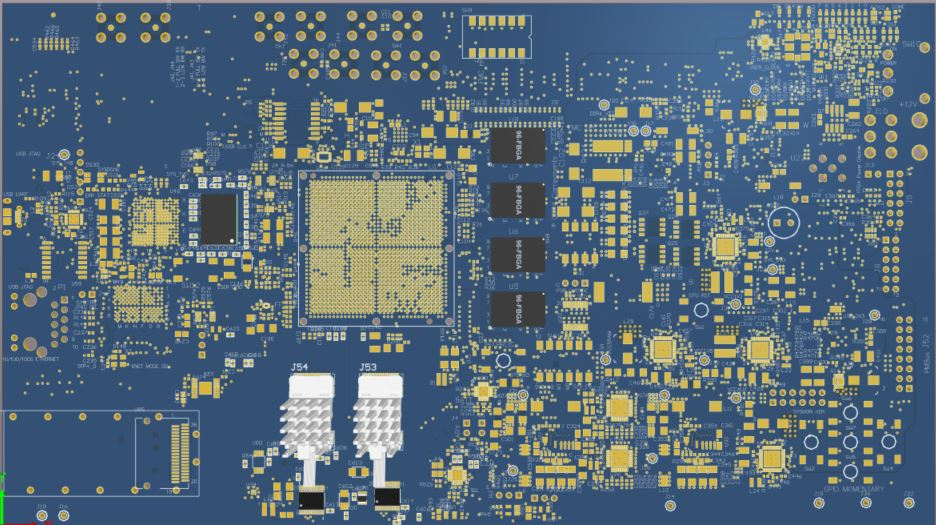
\includegraphics[width=1\textwidth]{board_3D_altium.png}
\caption{Altium 3D represantation of the board}
\label{fig1}
\end{figure}

\subsection{PCB}
Plated-through hole (PTH) via structures in high layer-count printed circuit boards (PCBs) can significantly distort high speed digital signals that pass through them. Often the  distortion is severe enough that digital receivers can no longer ascertain whether a  logical one or a logical zero was originally transmitted. 

\begin{figure}
\centering
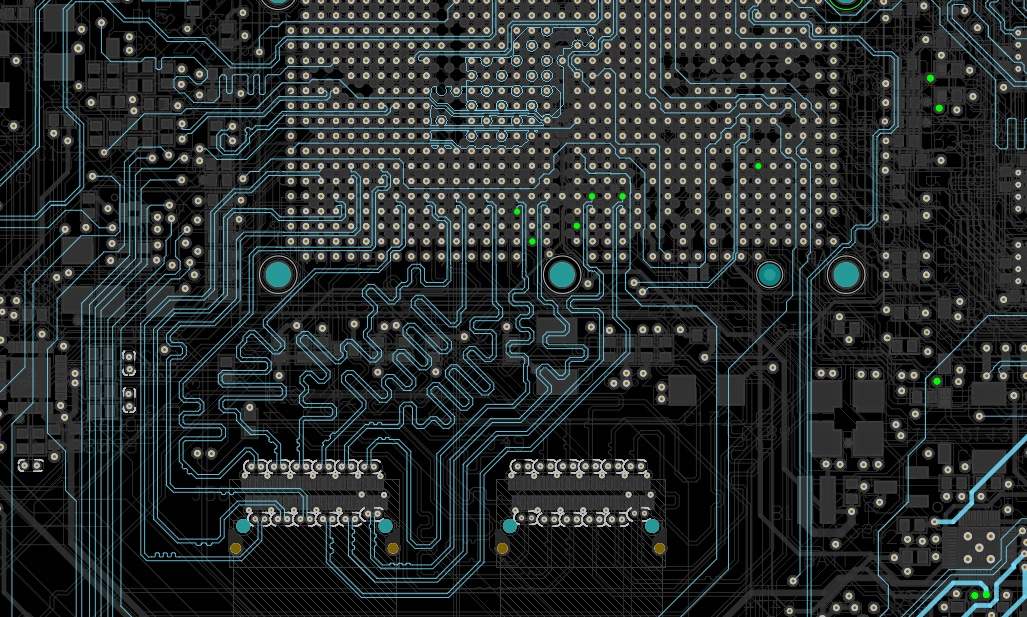
\includegraphics[width=0.5\textwidth]{serpentine_routing.png}
\caption{Serpentine routing of high speed differential signals}
\label{fig2}
\end{figure}


\end{document}

